\documentclass[10pt,twocolumn]{article}

\usepackage[T1]{fontenc}
\usepackage[utf8]{inputenc}
\usepackage{lmodern}
\usepackage{microtype}
\usepackage[a4paper,margin=2.0cm,columnsep=0.7cm]{geometry}
\usepackage{amsmath,amssymb}
\usepackage{booktabs}
\usepackage{graphicx}
\usepackage{listings}
\usepackage{url}
\usepackage[hidelinks]{hyperref}
\usepackage{tikz}
\usetikzlibrary{arrows.meta,positioning,fit,backgrounds,calc}

\lstset{
  basicstyle=\small\ttfamily,
  columns=fullflexible,
  keepspaces=true,
  frame=single,
  framesep=4pt,
  xleftmargin=2pt,
  breaklines=true
}

% ---- TikZ styles shared by all figures ----
\tikzset{
  cat/.style  = {draw, rounded corners=2pt, fill=black!4, inner sep=3pt,
                 font=\small, minimum height=5.5mm},
  item/.style = {draw, rounded corners=2pt, fill=blue!8, inner sep=3pt,
                 font=\small, minimum height=5.5mm},
  root/.style = {draw, circle, fill=black!10, inner sep=2pt, font=\small},
  qcat/.style = {cat, draw=orange!80!black, thick, fill=orange!12},
  hit/.style  = {item, draw=blue!60!black, thick, fill=blue!18},
  e/.style    = {-{Stealth[length=2mm]}, semithick},
  bad/.style  = {-{Stealth[length=2mm]}, semithick, red!70!black, dashed},
  layer/.style= {draw, rounded corners=3pt, minimum width=0.88\columnwidth,
                 align=center, inner sep=6pt, font=\small},
  note/.style = {font=\footnotesize\itshape, text=black!60, align=left}
}

\title{\textbf{OntoDAG: A Semantic Layer for Distributed Storage}}
\author{P\'eter F\"oldi\'ak\\
\small\texttt{peter.foldiak@gmail.com}\\
\small\url{https://github.com/petfold/ontodag}}
\date{}

\begin{document}
\maketitle

\begin{abstract}
Content-addressed storage networks such as Ethereum Swarm solve integrity
and availability, but they say nothing about \emph{meaning}: a 32-byte
reference does not tell you what a piece of content is, and the manifests
layered on top of it reproduce the fifty-year-old directory tree, which
forces every object into exactly one place. We present \textbf{OntoDAG}, a
multi-parent category DAG that acts as a semantic layer for decentralized
storage. Items are stored under any number of categories, and a single
query primitive returns everything below \emph{all} of a set of categories.
Because the transitive reduction of a DAG is unique, a correctly maintained
OntoDAG has exactly one canonical form; combined with a deterministic
encoding, the same knowledge always hashes to the same root reference.
This makes versions immutable snapshots, makes structural diffs cheap, and
lets concurrent, uncoordinated writers merge convergently in the manner of
a CRDT, so personal categories can extend shared ontologies without
corrupting them. Finally, we show how the category structure itself can be
\emph{learned} from data by the minimum description length (MDL) principle:
a concept is admitted only if it compresses the data enough to pay for its
own description. Learned categories are regenerable, so in Swarm's
postage-stamp economy they behave like a cache --- kept warm only while
query traffic justifies their storage rent. A Python implementation of the
data structure, its persistence layer, and its Swarm adapter is open
source and has been validated against a live Bee node on Gnosis mainnet.
\end{abstract}

\section{Introduction}

Decentralized storage has made remarkable progress on the questions of
\emph{where} and \emph{whether}: content addressing guarantees that a
reference identifies exactly one immutable byte string
\cite{merkle1987,benet2014}, and networks such as Ethereum Swarm
\cite{tron2020} add incentivized availability, mutable pointers (feeds),
and payment for storage (postage stamps). What none of this provides is an
answer to \emph{what}: what is this content, what is it about, how does it
relate to everything else I have stored? A hash is the perfect name for a
machine and the worst possible name for a mind.

The conventional answer is a manifest: a mapping from path names to
references --- in other words, a directory tree. But the directory tree is
an abstraction inherited from physical filing, and it systematically
under-describes content: every object must live in exactly one place, even
though almost everything we store is legitimately \emph{several things at
once}. The relational database, the other dominant organizational tool
\cite{codd1970}, fails for the complementary reason: its fixed columns
suit large collections of homogeneous records, not an open-ended universe
of heterogeneous things. What is missing between the two is a
\emph{semantic layer}: a small, principled structure that records what
things are, independently of where their bytes live.

This paper describes OntoDAG \cite{ontodag}, a semantic layer designed
specifically for content-addressed storage. It makes four contributions:

\begin{enumerate}
  \item \textbf{A minimal data structure} (Section~\ref{sec:ontodag}): a
  multi-parent category DAG with two primitives ---
  \texttt{put} an item under a set of categories, \texttt{get} the
  intersection of the categories' descendants --- maintained in
  transitively reduced form, which is provably unique
  \cite{aho1972} and therefore canonical.
  \item \textbf{A persistence mapping onto Swarm}
  (Section~\ref{sec:swarm}): one record per node in a canonically encoded
  trie, so that the same graph always yields the same root hash; commits
  are atomic root swaps, versions are free, and structural sharing makes
  updates proportional to the change, not to the graph.
  \item \textbf{Coordination-free multi-writer merge}
  (Section~\ref{sec:crdt}): defining the canonical state as the transitive
  reduction of the union of asserted edges makes concurrent updates
  commutative and idempotent --- the defining properties of a
  conflict-free replicated data type \cite{shapiro2011}.
  \item \textbf{A learning loop} (Sections~\ref{sec:mdl}--\ref{sec:econ}):
  categories can be proposed automatically by a minimum description length
  learner \cite{mdlfca}, and because learned categories are regenerable,
  Swarm's storage economics gives them a natural lifecycle --- they are a
  cache, priced by postage.
\end{enumerate}

The intended audience of this paper is developers of decentralized
systems, not machine-learning specialists; we introduce the classification
and MDL background from first principles.

\section{Why trees and tables are not enough}
\label{sec:trees}

\begin{figure}[t]
\centering
\resizebox{\columnwidth}{!}{%
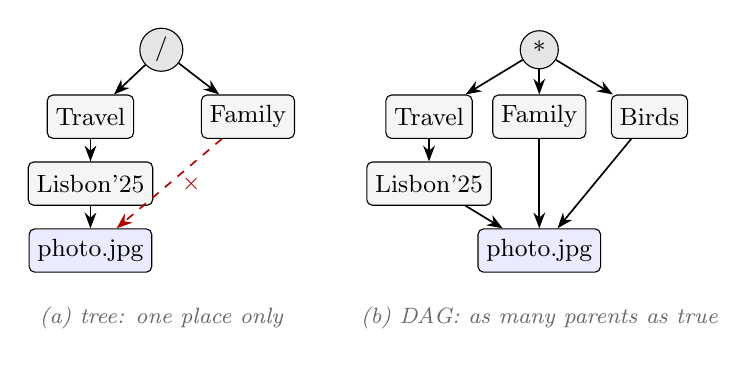
\begin{tikzpicture}[x=1cm,y=0.85cm]
  % ---- left: tree ----
  \node[root] (r1) at (1.5,3) {/};
  \node[cat] (tr) at (0.6,2) {Travel};
  \node[cat] (fa) at (2.6,2) {Family};
  \node[cat] (li) at (0.6,1) {Lisbon'25};
  \node[item] (p1) at (0.6,0) {photo.jpg};
  \draw[e] (r1) -- (tr);
  \draw[e] (r1) -- (fa);
  \draw[e] (tr) -- (li);
  \draw[e] (li) -- (p1);
  \draw[bad] (fa) -- (p1) node[midway,right=1pt,font=\footnotesize] {$\times$};
  \node[note,anchor=north] at (1.5,-0.7) {(a) tree: one place only};

  % ---- right: DAG ----
  \node[root] (r2) at (6.3,3) {*};
  \node[cat] (tr2) at (4.9,2) {Travel};
  \node[cat] (fa2) at (6.3,2) {Family};
  \node[cat] (bi2) at (7.7,2) {Birds};
  \node[cat] (li2) at (4.9,1) {Lisbon'25};
  \node[item] (p2) at (6.3,0) {photo.jpg};
  \draw[e] (r2) -- (tr2);
  \draw[e] (r2) -- (fa2);
  \draw[e] (r2) -- (bi2);
  \draw[e] (tr2) -- (li2);
  \draw[e] (li2) -- (p2);
  \draw[e] (fa2) -- (p2);
  \draw[e] (bi2) -- (p2);
  \node[note,anchor=north] at (6.3,-0.7) {(b) DAG: as many parents as true};
\end{tikzpicture}}
\caption{A photograph of a seagull taken on a family trip is
\emph{simultaneously} travel, family, and birds. A directory tree forces a
choice; a multi-parent DAG records all three memberships, and the item
becomes findable from every direction.}
\label{fig:treevsdag}
\end{figure}

\paragraph{Directory trees.}
A tree admits exactly one path to every object, so filing means choosing
\emph{the} place a thing belongs --- a choice that is almost always a
distortion (Figure~\ref{fig:treevsdag}). Is the photo from the family trip
filed under \texttt{Travel/Lisbon} or under \texttt{Family}? Whichever is
chosen, the other access path is destroyed. Symbolic links and shortcuts
are ad-hoc apologies for this defect, unmanaged and invisible to queries.
The deeper problem is that a tree conflates two independent questions ---
where content is stored and what it means --- which is precisely the
coupling content addressing was supposed to remove.

\paragraph{Flat tags.}
Tagging fixes multiple membership but discards structure: tags have no
relationship \emph{to each other}. A search for \texttt{bird} does not
return items tagged \texttt{penguin}, because nothing records that a
penguin is a bird. Every query must enumerate synonyms and
specializations by hand, and the tag vocabulary drifts into an
unmaintainable soup.

\paragraph{Relational tables.}
The relational model \cite{codd1970} is superb for large sets of
homogeneous records, but its fixed columns are the wrong shape for
describing an open universe of heterogeneous things. A car advertisement,
a holiday photo, a research paper, and a membership certificate do not
share a schema; modelling them relationally means either a table per kind
(with the taxonomy frozen into DDL) or a sparse mega-table of NULLs.
Moreover, subsumption --- the single most useful semantic relation,
``every X is a Y'' --- is not a join; SQL can store it but cannot
naturally query with it.

\paragraph{Hierarchical and faceted classification.}
Library science met this problem a century before file systems.
\emph{Hierarchical} schemes such as Dewey give a single deep taxonomy ---
navigable and browsable, but again one shelf position per book.
\emph{Faceted} classification, introduced by Ranganathan's Colon
Classification \cite{ranganathan1933}, instead describes an object by
independent aspects (his classics: personality, matter, energy, space,
time; a modern e-commerce equivalent: product type $\times$ region
$\times$ price band $\times$ condition). Facets compose --- ``electric
\emph{cars} in \emph{Germany}'' --- without anyone having pre-built that
shelf. But facets alone are not enough either, because each facet is
itself hierarchical: \emph{Germany} sits inside \emph{Europe},
\emph{electric} inside \emph{powertrain}. What is actually needed is the
combination: \textbf{multiple, individually hierarchical facets, whose
combinations are formed on demand at query time}. Formally, categories
ordered by subsumption with multiple parents form a lattice rather than a
tree; Formal Concept Analysis (FCA) \cite{wille1982,ganter1999} studies
exactly these structures, and we return to it in Section~\ref{sec:mdl} as
the mathematical basis of \emph{learning} categories. The data structure
that represents such an order with no redundancy is a directed acyclic
graph --- which is what OntoDAG is.

\section{OntoDAG: the data structure}
\label{sec:ontodag}

OntoDAG \cite{ontodag} is a deliberately minimal, subsumption-only
ontology: a multi-parent category DAG with one insertion primitive and one
query primitive. In the spirit of Bush's associative memory
\cite{bush1945}, everything is reachable by what it \emph{is} rather than
by where it was put.

\paragraph{Structure.}
Nodes are \emph{items}. There is intentionally no separate notion of
``class'' versus ``instance'': any instance can later be subdivided (a
book $\to$ an edition $\to$ my copy $\to$ my copy when new), so no
principled boundary exists, and OntoDAG does not pretend to draw one. An
item that tags stored content simply carries a payload reference. Edges
mean subsumption: an edge $A \to B$ asserts that $B$ is a kind of (or an
instance of, or a part of the extension of) $A$. A distinguished root
\texttt{*} is the implicit ancestor of everything.

\paragraph{The two primitives.}
\begin{itemize}
  \item $\texttt{put}(x, \{S_1,\dots,S_k\})$ --- insert item $x$ under
  supercategories $S_1,\dots,S_k$.
  \item $\texttt{get}(\{C_1,\dots,C_k\}) \;=\; \bigcap_{i=1}^{k}
  \mathrm{desc}(C_i)$ --- return every item below \emph{all} of the query
  categories, where $\mathrm{desc}(C)$ is the set of descendants of $C$.
\end{itemize}
That is the whole interface. A query is a conjunction of facets, and the
answer is the intersection of their descendant cones
(Figure~\ref{fig:putget}).

\begin{figure}[t]
\centering
\resizebox{\columnwidth}{!}{%
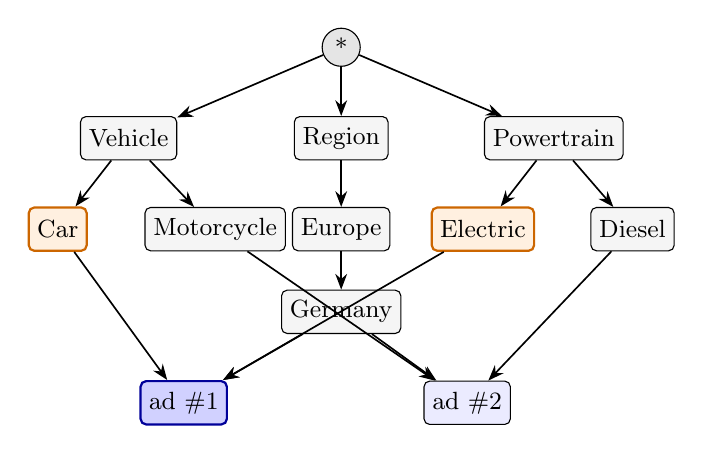
\begin{tikzpicture}[x=1cm,y=1.05cm]
  \node[root] (r) at (4.2,3.3) {*};
  \node[cat]  (veh) at (1.5,2.2) {Vehicle};
  \node[cat]  (reg) at (4.2,2.2) {Region};
  \node[cat]  (pow) at (6.9,2.2) {Powertrain};
  \node[qcat] (car) at (0.6,1.1) {Car};
  \node[cat]  (mot) at (2.6,1.1) {Motorcycle};
  \node[cat]  (eur) at (4.2,1.1) {Europe};
  \node[qcat] (ele) at (6.0,1.1) {Electric};
  \node[cat]  (die) at (7.9,1.1) {Diesel};
  \node[cat]  (ger) at (4.2,0.1) {Germany};
  \node[hit]  (a1) at (2.2,-1.0) {ad \#1};
  \node[item] (a2) at (5.8,-1.0) {ad \#2};
  \draw[e] (r) -- (veh); \draw[e] (r) -- (reg); \draw[e] (r) -- (pow);
  \draw[e] (veh) -- (car); \draw[e] (veh) -- (mot);
  \draw[e] (reg) -- (eur); \draw[e] (eur) -- (ger);
  \draw[e] (pow) -- (ele); \draw[e] (pow) -- (die);
  \draw[e] (car) -- (a1); \draw[e] (ger) -- (a1); \draw[e] (ele) -- (a1);
  \draw[e] (mot) -- (a2); \draw[e] (ger) -- (a2); \draw[e] (die) -- (a2);
\end{tikzpicture}}
\caption{A miniature car-market OntoDAG (taken from the reference
implementation's demo). Listings were inserted with
$\texttt{put}(\text{ad\#1}, \{\text{Car},\text{Germany},\text{Electric}\})$
and $\texttt{put}(\text{ad\#2},
\{\text{Motorcycle},\text{Germany},\text{Diesel}\})$. The query
$\texttt{get}(\{\text{Car},\text{Electric}\})$ (highlighted categories)
intersects the two descendant cones and returns ad~\#1 (highlighted item)
--- no ``electric cars'' category was ever created.}
\label{fig:putget}
\end{figure}

\paragraph{Canonical form: the transitive reduction.}
The stored graph is kept \emph{transitively reduced}: if a path
$A \to B \to C$ exists, the direct edge $A \to C$ must not. Redundant
supercategory links are pruned automatically --- if a user writes
$\texttt{put}(\text{penguin}, \{\text{Bird}, \text{Animal}\})$ while
$\text{Bird}$ is already below $\text{Animal}$, the
$\text{Animal}\to\text{penguin}$ edge is dropped as implied. The decisive
mathematical fact is that \textbf{the transitive reduction of a DAG is
unique} \cite{aho1972}. Uniqueness means a correctly maintained OntoDAG has
exactly \emph{one} form regardless of the order or history of insertions:
the graph is a pure function of the knowledge it encodes. The reference
implementation enforces this with a machine-checked invariant suite ---
acyclicity, exact transitive reduction, insertion-order independence,
consistency of cached descendant counts, and a commutative, idempotent
\texttt{merge} --- because, as Section~\ref{sec:swarm} shows, the entire
persistence and multi-writer story rests on canonicality being exact
rather than approximate.

\paragraph{Relationship to ontologies.}
OntoDAG sits deliberately between flat tags and full ontology stacks. It
is an ontology in Gruber's sense --- an explicit specification of a
conceptualization \cite{gruber1993} --- but it keeps only the taxonomic
backbone: the subsumption order, which in OWL terms is the
\texttt{subClassOf} skeleton \cite{owl2}. It omits properties, axioms,
restrictions, and description-logic reasoning, and in exchange its one
query primitive is cheap, predictable, and needs no reasoner. The
reference implementation imports and exports OWL class hierarchies
(including Manchester syntax), so existing ontologies can seed an OntoDAG
and curated OntoDAGs can flow back to standard tools.

\section{Persistence on Swarm}
\label{sec:swarm}

\begin{figure}[t]
\centering
\resizebox{0.97\columnwidth}{!}{%
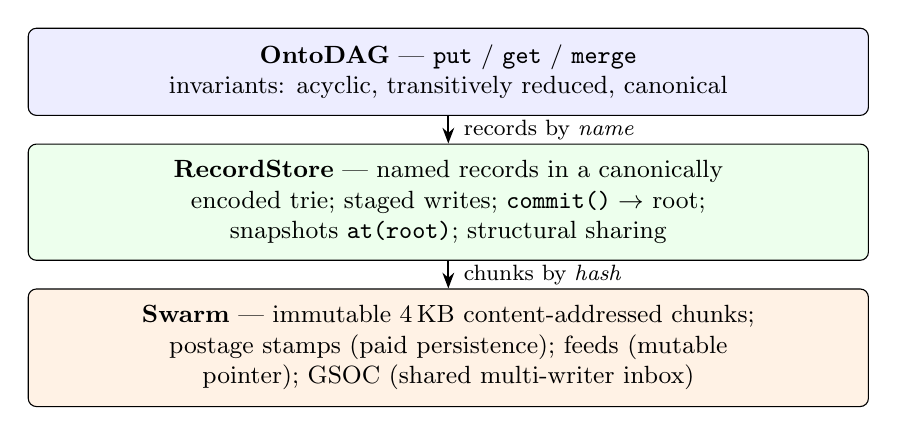
\begin{tikzpicture}[node distance=3.5mm]
  \node[layer, fill=blue!7] (onto)
    {\textbf{OntoDAG} --- \texttt{put} / \texttt{get} / \texttt{merge}\\
     invariants: acyclic, transitively reduced, canonical};
  \node[layer, fill=green!7, below=of onto] (rs)
    {\textbf{RecordStore} --- named records in a canonically\\
     encoded trie; staged writes; $\texttt{commit()} \to$ root;\\
     snapshots \texttt{at(root)}; structural sharing};
  \node[layer, fill=orange!10, below=of rs] (swarm)
    {\textbf{Swarm} --- immutable 4\,KB content-addressed chunks;\\
     postage stamps (paid persistence); feeds (mutable\\
     pointer); GSOC (shared multi-writer inbox)};
  \draw[e] (onto) -- node[right=2pt,font=\footnotesize] {records by \emph{name}} (rs);
  \draw[e] (rs) -- node[right=2pt,font=\footnotesize] {chunks by \emph{hash}} (swarm);
\end{tikzpicture}}
\caption{The three-layer architecture. Graph semantics exist only in the
top layer; the record store knows nothing about edges or descendants and
is reusable for any versioned key--value data; the bottom layer is the
public Swarm network. Each layer talks to the next through a narrow
interface, so storage-layout changes (chunk packing, batching) never
touch graph code.}
\label{fig:stack}
\end{figure}

\subsection{Swarm in one paragraph}
Ethereum Swarm \cite{tron2020} is a peer-to-peer storage network whose
atomic unit is an immutable 4\,KB \emph{chunk}, addressed by the hash of
its content. Arbitrary-length payloads are split into Merkle trees of
chunks behind a single 32-byte reference. Storage is paid for with
\emph{postage stamps} --- prepaid, on-chain batches that entitle chunks to
live in the network until the batch's value is exhausted; unstamped or
expired chunks are eventually garbage-collected. \emph{Feeds} provide
mutability: a single-owner, signed pointer that can be updated to
reference the latest immutable state. \emph{GSOC} (Graffiti Several
Owner Chunks) generalizes this into a shared address to which many
parties can post signed messages --- a decentralized inbox we will use in
Section~\ref{sec:crdt}.

\subsection{Why the fit is unusually good}
Content-addressed immutable storage merges two senses of ``persistent''
that normally have to be engineered separately: \emph{durable} (the
database sense) and \emph{immutable with structural sharing} (the
functional-programming sense, as in Git or Ethereum's state trie). For
most data structures this is merely convenient. For OntoDAG it is
foundational, because of the canonical form: since the graph is a pure
function of its content, and the encoding below is deterministic,
\textbf{the same knowledge always hashes to the same root reference}.
Consequences, in decreasing order of obviousness:

\begin{itemize}
  \item \textbf{Versions are free.} Every \texttt{commit} yields a new
  root; old roots remain valid, self-consistent snapshots forever. History
  is a by-product, not a feature to build.
  \item \textbf{Diffs are cheap.} Two roots share every unchanged subtree
  by construction, so comparing versions touches only what differs ---
  the Merkle-tree argument \cite{merkle1987} applied to an ontology.
  \item \textbf{Equality is a hash comparison.} Two parties can verify
  they hold the same ontology --- however differently they arrived at it
  --- by comparing 32 bytes. This is the property the multi-writer story
  in Section~\ref{sec:crdt} cashes in.
\end{itemize}

\subsection{The RecordStore layer}
Between the graph and the chunk store sits a deliberately generic layer
(Figure~\ref{fig:stack}): a versioned key$\to$record store over any
content-addressed chunk backend. It contributes exactly what Swarm does
not natively provide: typed records rather than raw references; a
\emph{canonical codec} (sorted keys, fixed separators --- a correctness
requirement, since any encoding nondeterminism would break
same-content-same-root); \emph{atomic commits} (an OntoDAG \texttt{put}
touches several records --- the new node, its parents' edge lists ---
and \texttt{commit()} lands them as one new root, so no reader ever sees a
torn write); and \emph{snapshot isolation} (a reader pins one root and
traverses a frozen, self-consistent dataset with no locking). Keys live in
a compacted radix trie whose nodes are themselves canonically encoded
chunks, giving structural sharing: in the test suite, updating 1 of 200
records writes fewer than 12 new chunks.

One OntoDAG node maps to one record, keyed by its name:

\begin{lstlisting}
"Germany": {
  "up":    ["Europe"],          // parents, sorted
  "down":  ["ad#1", "ad#2"],    // children, sorted
  "count": 2,                   // descendants
  "payload": null,              // optional Swarm ref
  "meta":  {}                   // optional, e.g. type
}
\end{lstlisting}

A typical record is 300--500 bytes; hub nodes with thousands of edges
exceed a chunk, but Swarm's splitter already turns any payload into a
chunk tree behind one reference, so the schema stays flat.

\subsection{Performance model}
The dominant cost is the network chunk fetch, not any code-level choice: a
chunk on the local Bee node costs 1--5\,ms, a cold chunk fetched across
the network 100--500\,ms --- four to six orders of magnitude above an
in-memory pointer hop. Two facts make this workable. First, immutable
chunks \emph{cache perfectly}: no invalidation is ever needed, at any
layer (in-process, the local Bee store, HTTP caches downstream). Second,
ontologies are small relative to the content they organize --- a
100{,}000-node OntoDAG is a few tens of megabytes --- so the practical
pattern is \emph{hydrate once, query in RAM, commit mutations for
durability and sync}. Partial, on-demand loading through the trie is the
regime for graphs that outgrow memory, and the layering of
Figure~\ref{fig:stack} confines that change below the record interface.

\subsection{Implementation status}
The full stack of Figure~\ref{fig:stack} is implemented in Python and open
source \cite{ontodag}: the invariant-checked data structure, the record
store (unit-tested and model-based-fuzzed against a dictionary oracle,
including the canonical-root property under arbitrary put/delete
histories), and the \texttt{SwarmOntoDAG} adapter (13 tests, including
merge convergence to bit-identical roots). The chunk backend has passed
its integration suite against a live Bee v2.8.1 light node on Gnosis
mainnet with a real purchased postage batch.

\section{Concurrent writers without coordination}
\label{sec:crdt}

\begin{figure}[t]
\centering
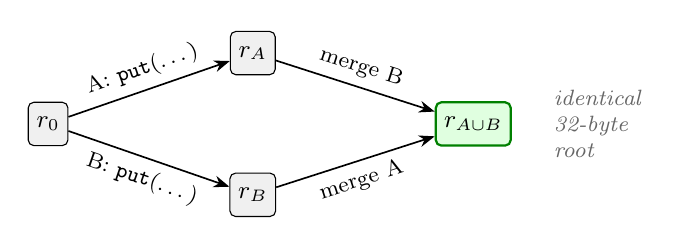
\begin{tikzpicture}[x=1cm,y=1.0cm]
  \node[cat, fill=black!6] (r0) at (0,0) {$r_0$};
  \node[cat, fill=black!6] (ra) at (2.6,0.9) {$r_A$};
  \node[cat, fill=black!6] (rb) at (2.6,-0.9) {$r_B$};
  \node[cat, fill=green!12, draw=green!50!black, thick] (rm) at (5.4,0) {$r_{A\cup B}$};
  \draw[e] (r0) -- node[above,sloped,font=\footnotesize] {A: \texttt{put}(\dots)} (ra);
  \draw[e] (r0) -- node[below,sloped,font=\footnotesize] {B: \texttt{put}(\dots)} (rb);
  \draw[e] (ra) -- node[above,sloped,font=\footnotesize] {merge B} (rm);
  \draw[e] (rb) -- node[below,sloped,font=\footnotesize] {merge A} (rm);
  \node[note, anchor=west] at (6.3,0) {identical\\32-byte\\root};
\end{tikzpicture}
\caption{Convergent merge. Writers A and B extend the same snapshot $r_0$
independently; whichever order the merges happen in --- and however many
times they are repeated --- both replicas reach the \emph{same} root
reference, verifiable by comparing hashes. No coordinator, no lock, no
conflict dialog.}
\label{fig:merge}
\end{figure}

Git taught a generation of developers that immutable snapshots plus merge
beat locks --- but Git merges can conflict, because arbitrary text has no
merge rule. OntoDAG's canonical form supplies one. Define the canonical
state of a replicated OntoDAG as
\[
  G \;=\; \mathrm{TR}\!\left(\;\bigcup_{w \in \text{writers}} E_w\right),
\]
the transitive reduction of the union of all asserted edges. Union is
commutative, associative, and idempotent, and $\mathrm{TR}$ is a unique
normal form \cite{aho1972} --- so concurrent \texttt{put} operations from
independent writers can be applied in any order, or repeatedly, and every
replica converges to the same graph and hence (via the canonical encoding)
to the same root hash (Figure~\ref{fig:merge}). These are precisely the
convergence conditions of state-based CRDTs \cite{shapiro2011}. Removal,
as always in CRDT territory, needs care: a plain delete does not commute
with a concurrent re-add, so removals carry observed-remove tombstones.

The planned transport is Swarm-native: writers post signed operations
($\texttt{put}(name, supers)$, $\texttt{remove}(name)$) to a shared GSOC
address, and any reader deterministically folds the pending operation set
into the current root and publishes the result on a feed. Because folding
is deterministic, it does not matter \emph{who} folds --- any two folders
produce bit-identical roots.

The payoff for users is the local-first property \cite{kleppmann2019}:
\textbf{personal categories extend shared ontologies without corrupting
them}. A community can maintain a shared base taxonomy (say, the car
market of Figure~\ref{fig:putget}); an individual layers private
categories over it (\emph{my shortlist}, \emph{seen at the dealer});
merge semantics guarantee the overlay never damages the base, and the
base can be upgraded under the overlay by the same union-and-reduce rule.

\section{Where do categories come from? Learning by compression}
\label{sec:mdl}

Everything so far assumes someone \emph{asserts} the categories. Manual
curation is exactly right for personal, deliberate structure, but it does
not scale to large corpora, and it never discovers the categories you did
not think to create. The mathematical home of ``categories latent in
data'' is Formal Concept Analysis \cite{wille1982,ganter1999}: given a
binary object$\times$attribute table, FCA derives all \emph{concepts} ---
maximal sets of objects sharing a maximal set of attributes --- ordered by
subsumption into a lattice: multi-parent, acyclic, downward-closed --- the
same shape as an OntoDAG. FCA's classical defect is that it is
\emph{too} faithful: the number of formal concepts can grow exponentially,
and most of them are coincidences of the sample rather than structure
worth keeping.

The minimum description length (MDL) principle
\cite{rissanen1978,grunwald2007} supplies the missing filter, and it can
be stated entirely in terms a systems audience already trusts:
\textbf{the best model of your data is the one that compresses it best,
where the model's own description counts against it}. Formally, choose the
concept DAG $G$ minimizing
\[
  L(G) \;+\; L(D \mid G),
\]
the bits to describe the model plus the bits to describe the data given
the model. A candidate concept (say, \emph{German electric car}) earns a
place in the DAG only if factoring it out shortens the total description:
each object covered by it can then be described as ``one of those, plus
these deviations,'' and the saving must exceed the cost of writing the
concept down (Figure~\ref{fig:mdl}). Rare coincidences never pay for themselves; genuine
regularities always do, given enough data. This is not an analogy ---
compression and prediction are formally two views of the same quantity ---
but the practical reading is the honest one: \emph{MDL is a principled,
parameter-free answer to ``is this category worth keeping?''}

\begin{figure}[t]
\centering
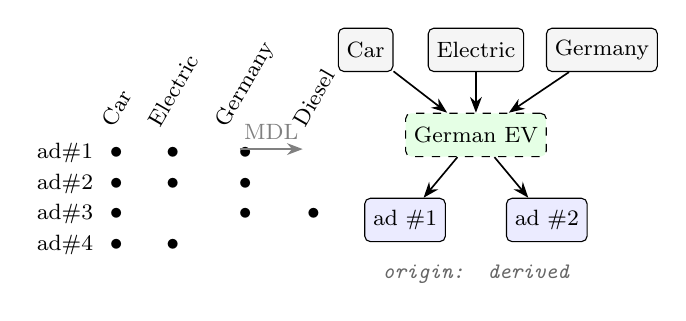
\begin{tikzpicture}[x=1cm,y=0.9cm]
  % ---- left: object x attribute context ----
  \node[font=\small, anchor=west] (tbl) at (-0.4,1.0) {%
    \begin{tabular}{@{}l@{\;}c@{\;\;}c@{\;\;}c@{\;\;}c@{}}
      & \rotatebox{60}{\footnotesize Car}
      & \rotatebox{60}{\footnotesize Electric}
      & \rotatebox{60}{\footnotesize Germany}
      & \rotatebox{60}{\footnotesize Diesel} \\
      \footnotesize ad\#1 & $\bullet$ & $\bullet$ & $\bullet$ & \\
      \footnotesize ad\#2 & $\bullet$ & $\bullet$ & $\bullet$ & \\
      \footnotesize ad\#3 & $\bullet$ &           & $\bullet$ & $\bullet$ \\
      \footnotesize ad\#4 & $\bullet$ & $\bullet$ &           & \\
    \end{tabular}};
  \draw[e, black!50] (2.3,1.0) -- node[above,font=\footnotesize]{MDL} (3.1,1.0);
  % ---- right: learned concept in the DAG ----
  \node[cat] (car) at (3.9,2.4) {\footnotesize Car};
  \node[cat] (ele) at (5.3,2.4) {\footnotesize Electric};
  \node[cat] (ger) at (6.9,2.4) {\footnotesize Germany};
  \node[cat, dashed, fill=green!10] (gev) at (5.3,1.2) {\footnotesize German EV};
  \node[item] (b1) at (4.4,0.0) {\footnotesize ad \#1};
  \node[item] (b2) at (6.2,0.0) {\footnotesize ad \#2};
  \draw[e] (car) -- (gev); \draw[e] (ele) -- (gev); \draw[e] (ger) -- (gev);
  \draw[e] (gev) -- (b1); \draw[e] (gev) -- (b2);
  \node[note, anchor=north] at (5.3,-0.5) {\texttt{origin: derived}};
\end{tikzpicture}
\caption{Learning a category by compression. The attribute combination
\{Car, Electric, Germany\} recurs in the object$\times$attribute data
(left), so factoring it out as a concept shortens the total description:
the learner inserts a \emph{German EV} node (dashed) into the DAG, and the
covered items are described through it. A combination that occurred once
would not pay for its own description and is never materialized.}
\label{fig:mdl}
\end{figure}

The companion project \textbf{mdl-fca} \cite{mdlfca} implements this
program: a greedy pair-merge constructor proposes candidate concepts and a
search framework keeps those that pay their way, in both batch and online
settings. Crucially, its output DAG is structurally aligned with OntoDAG
--- downward-closure semantics, multiple parents, acyclic --- so a learned
DAG becomes an OntoDAG snapshot through an essentially identity
conversion, and everything in Sections~\ref{sec:swarm}--\ref{sec:crdt}
(canonical roots, snapshots, merge) applies to learned structure
unchanged. The learner remains a separate package that depends on OntoDAG
as a library, so learners are swappable and the core stays dependency-free.

\section{Learned categories are a cache: MDL meets storage economics}
\label{sec:econ}

Mixing hand-asserted and machine-proposed structure in one graph raises an
obvious worry: which nodes can you trust, and which can you afford to
lose? The answer is not an instance/class distinction (rejected in
Section~\ref{sec:ontodag}) but \emph{provenance}, orthogonal to what a
node is:

\begin{itemize}
  \item \texttt{origin: asserted} --- placed by an external act (a user,
  an import, an observation). Ground truth; not regenerable; losing it is
  data loss.
  \item \texttt{origin: derived} --- proposed by a learner because it
  compressed asserted data. A pure function of (corpus, learner); pinned
  as \texttt{derived\_from = (corpus\_root, learner\_version)}, where the
  corpus root is itself a content-addressed snapshot. Losing it is only a
  cache miss.
  \item \texttt{endorsed} --- a user may promote a derived concept they
  have come to rely on; re-learning may propose a replacement but must not
  silently overwrite an endorsed node.
\end{itemize}

This single bit is where the learning story and the storage economics
click together. Swarm charges rent per chunk via postage stamps
(Section~\ref{sec:swarm}); every node record is a chunk; so every category
has a carrying cost. Provenance says which costs are obligatory:
\textbf{asserted nodes must stay stamped and pinned regardless; derived
nodes are kept warm only while query traffic justifies their postage},
and are otherwise allowed to expire and be recomputed on demand ---
\emph{exactly} the economics of a cache, applied to knowledge. The same
bit routes synchronization in the shared/personal architecture of
Section~\ref{sec:crdt} (Table~\ref{tab:2x2}): the big shared base is
largely derived and therefore cheap to distribute (peers with the corpus
recompute it and sync only diffs), while personal assertions are the
small, irreplaceable payload that deserves durable stamps and backup.

\begin{table}[t]
\centering
\footnotesize
\setlength{\tabcolsep}{4pt}
\begin{tabular}{@{}lll@{}}
\toprule
 & \textbf{shared} & \textbf{personal} \\
\midrule
\textbf{asserted} & curate, stamp durably & back up; irreplaceable \\
\textbf{derived}  & recompute from corpus; & recompute per device; \\
                  & sync diffs only        & let postage lapse \\
\bottomrule
\end{tabular}
\caption{Provenance $\times$ ownership routes what must be stored durably
versus what may be lazily recomputed.}
\label{tab:2x2}
\end{table}

There is also a genuinely new research question here, which we record
without claiming to have solved it. Classical MDL scores a concept by how
often it helps \emph{generate} the data. In a metered, separately-queried
store, a concept also has a \emph{retrieval} value --- how often queries
actually read it --- which is a property of the workload, not the corpus.
The natural extension is
\[
  L(G) + L(D \mid G) \;+\; \lambda \sum_{c \in G}
  f_{\mathrm{ret}}(c)\, \cdot\, s(c),
\]
where $f_{\mathrm{ret}}$ comes from the query log, $s(c)$ is the storage
cost of keeping $c$ warm, and $\lambda$ (bits per byte-second) prices
storage against description length. The term vanishes in the in-memory
setting and collapses when the query distribution mirrors the data --- but
personal tools are exactly where the two diverge, as users repeatedly
query their statistically-rare pet categories. Retrieval-aware MDL would
let the learner itself decide which categories deserve postage.

\section{Status and future work}
\label{sec:status}

Implemented and tested \cite{ontodag}: the invariant-checked core
(acyclicity, unique transitive reduction, order independence, iterative
traversals, commutative idempotent merge); the record store with canonical
roots verified by model-based fuzzing; the Swarm adapter with
merge-convergence-to-identical-roots tests; OWL import/export; a REST API
and web demo; Bee integration validated on Gnosis mainnet (v2.8.1, real
postage batch). Open, in planned order: network-level retrievability and
pinning checks; the GSOC operation log and fold rule of
Section~\ref{sec:crdt} (the in-memory merge algebra it needs is already
tested); a signed feed pointer; chunk-packing and batched fetches (behind
the existing interface, driven by usage data rather than speculation); and
the mdl-fca integration with the provenance schema of
Section~\ref{sec:econ}.

\section{Conclusion}

The organizational layer of storage has lagged its transport layer by
decades: we address content by cryptographic hash and then file it in a
tree from 1970. OntoDAG proposes a small correction with large
consequences. A subsumption-only, multi-parent category DAG is expressive
enough to combine hierarchical and faceted classification, yet simple
enough to have a \emph{canonical form} --- and on a content-addressed
network, canonical form is superpower: identical knowledge gets identical
hashes, versions and diffs come for free, and uncoordinated writers
provably converge. The same structure is the natural output format of
compression-based concept learning, and Swarm's storage economics gives
learned categories precisely the lifecycle they deserve: asserted
knowledge is preserved like data, derived knowledge is priced like a
cache. Between the directory tree and the description-logic reasoner
there is a productive middle --- and it fits in 4\,KB chunks.

\paragraph{Acknowledgments.}
The reference implementation, its Swarm design document, and the mdl-fca
learner are open source at \url{https://github.com/petfold/ontodag} and
\url{https://github.com/petfold/mdl-fca}.

\begingroup
\small
\bibliographystyle{abbrv}
\bibliography{references}
\endgroup

\end{document}
